% =====================================================================================
%  paper.tex — Fe/MgO wetting paper, ported from the approved markdown sections (E2).
%
%  Source of truth (all APPROVED 2026-09-18):
%     sections/06_abstract.md  ->  abstract.tex
%     sections/04_introduction.md -> introduction.tex
%     sections/01_methods.md   ->  methods.tex
%     sections/02_results.md   ->  results.tex
%     sections/03_discussion.md -> discussion.tex
%     sections/05_conclusion.md -> conclusion.tex
%     sections/SI.md           ->  SI.tex   (separate supplementary document)
%
%  Port rules (AGENTS.md, Phase E2):
%    * \cite{} keys are carried over byte-for-byte from the markdown; no re-keying.
%    * Markdown pipe tables -> booktabs tabular; **bold** -> \textbf{}.
%    * Unicodes (ΔZ, eV/atom, κ, ≥, ×, −) -> LaTeX macros/math.
%    * The mermaid flowchart of Fig. 1 is re-drawn as TikZ.
%    * Figures 2 and 3 reference figures/*.png (300 dpi, produced by scripts/).
%
%  Standalone (venue-agnostic) preamble: swap in the target journal's class when the
%  venue is fixed — the \cite keys and content need no change.
%
%  NOTE: [TITLE] and the author block are placeholders — not yet fixed by the scientist.
%  NOTE: the markdown §1/§2/§3 numbering maps onto the final-manuscript II/III/IV
%        numbering used by the Introduction's roadmap.
% =====================================================================================
\documentclass[10pt]{article}
\usepackage[margin=1in]{geometry}
\usepackage{amsmath,amssymb}
\usepackage{booktabs}
\usepackage{graphicx}
\usepackage{siunitx}
\usepackage{tikz}
\usetikzlibrary{arrows.meta,positioning,fit,backgrounds,shapes.geometric}
\usepackage{hyperref}
\usepackage[numbers,sort&compress]{natbib}

\graphicspath{{figures/}}

% Sub-sub headings are numbered (they are the manuscript's paragraph-level headings).
\setcounter{secnumdepth}{3}
\setlength{\emergencystretch}{2em}

% Recurring shorthand.
\newcommand{\dZ}{\ensuremath{\Delta Z}}
\newcommand{\dEN}{\ensuremath{\Delta E/N}}
\newcommand{\eVA}{\ensuremath{\text{eV/atom}}}
\newcommand{\evpa}{\ensuremath{\text{eV/atom}}}

\title{Effect of boron insertion on metal-film wetting of Fe on MgO}
\author{Andi Muhammad Nur Fitrah Syamsul\thanks{Graduate School of Engineering, Mie University,
Tsu, Mie 514-8507, Japan.}\and Kohji Nakamura}
\date{\today}

\begin{document}

\maketitle

\begin{abstract}
% Ported from sections/06_abstract.md (v1, APPROVED 2026-09-18).
% Final-manuscript Abstract. No \cite{} (standard for an abstract).
The wetting of a metal film on MgO(001)---the interface at the heart of MgO-based magnetic tunnel
junctions---is governed by the competition between a flat, well-wetting film and a dewetted island.
We map this competition for the same Fe host with and without added boron, using a biased,
surrogate-driven search that targets the two configurations the wetting question is about. In both
models the island is the ground state, so the flat film is a distinct, higher-energy basin---by
0.1888~\eVA{} for Fe/MgO and by 0.1493~\eVA{} for Fe-B/MgO. Adding boron lowers the
flat--island separation by 0.040~\eVA, a 21\,\% reduction, at a search-level significance of
$p = 0.0444$, and boron acts inside the film rather than at the interface. Boron therefore moves the
flat, well-wetting configuration closer to the island ground state without displacing it---the
direction the confusion principle of metallic-glass formation predicts---and so favours the flat film
that MgO-based tunnel junctions require.

\end{abstract}

% Ported from sections/04_introduction.md (v11, APPROVED 2026-09-18).
% Continuous prose, no subsections. Final-manuscript Sec.~I.
\section{Introduction}
\label{sec:intro}

MgO-based magnetic tunnel junctions reach very large tunnel magnetoresistance at room temperature
when the barrier is crystalline and the metal electrodes are matched to it in-plane
\cite{yuasa2004,parkin2004}. The transport calculations that account for the effect were carried out
for an ideal Fe$|$MgO$|$Fe(001) interface, in which a flat metal layer sits directly above the
substrate oxygen \cite{butler2001}. Achieving those values in practice is a question of realising
that interface closely enough: the high magnetoresistance is obtained when the barrier is
(001)-oriented and the metal film flat and continuous \cite{yuasa2004}, and the barrier's
orientation and stress relaxation are themselves sensitive to how the metal is deposited and
annealed \cite{djayaprawira2005,ikeda2008}. The structural quality of the metal/oxide interface is
therefore part of the specification of the device rather than an incidental detail.

Two recent trends in junction fabrication have only sharpened that point. The first is the push on
the tunnel magnetoresistance itself: after a decade of stagnation at the 604\,\% reported in 2008
for junctions with boron-alloy electrodes \cite{ikeda2008}, epitaxial junctions now reach a record
631\,\% at room temperature (1143\,\% at 10~K), and the gain comes explicitly from the
interface---from tuning the crystallographic orientation and the oxygen content of the MgO barrier
through ultrathin metal insertions at the metal/oxide boundary \cite{scheike2023}. The second is the
move to perpendicularly magnetised junctions for dense, non-volatile memory, in which the
metal/oxide interface is itself a functional layer: the Fe/MgO interface carries a large
perpendicular surface anisotropy, whose strength is traced to the hybridisation of interfacial iron
and oxygen states \cite{solano2022}, and sub-nanometre metal films grown on the barrier are
engineered for the perpendicular anisotropy and the low magnetic damping that low-power switching
requires \cite{ichinose2025}. Both trends converge on the same requirement---a metal film that is
flat, epitaxial and well-wetting on the crystalline barrier---and, in practice, on layer-by-layer
control of the roughness and thickness of each film in the stack \cite{ghemes2024}.

The flat, lattice-matched film assumed in such interface models is not, however, the configuration
that a metal film necessarily adopts when it is deposited on MgO(001). At the monolayer coverages
relevant to a thin electrode, growth experiments find the film dewetting into three-dimensional
islands: He-atom scattering records three-dimensional island growth of Fe on MgO(001) at room
temperature, suppressed only when the film is deposited at 140~K \cite{fahsold2000}; scanning
tunnelling microscopy combined with X-ray magnetic circular dichroism finds sub-nanometre Fe growing
three-dimensionally, with a two-dimensional growth mode reported only above about 6.5 monolayers
\cite{torelli2009}; and grazing-incidence small-angle X-ray scattering on five monolayers likewise
identifies Volmer--Weber growth with spherical islands \cite{reitinger2007}. A flat, pseudomorphic
monolayer is obtained instead by slow deposition onto a cleaved, oxygen-annealed crystal
\cite{urano1988}. The islanding tendency survives even into the most controlled modern fabrication:
grain-to-grain epitaxial growth of a sub-nanometre ferromagnetic layer on a polycrystalline
MgO(001) barrier on 300\,mm wafers must be performed at cryogenic temperature (100~K), because
room-temperature deposition lets the metal nucleate as islands and break the film's continuity
\cite{ichinose2025}. Two structural outcomes thus compete at this coverage---a flat, well-wetting
film and a dewetted island---and the growth experiments constrain their kinetics rather than their
relative energies, while interface models assume the flat geometry by construction. What is missing
is a comparison of the two configurations' energies for one and the same interface, and an answer to
how that comparison responds to a change in the film's composition.

The composition is not arbitrary. The metal electrodes of the highest-magnetoresistance MgO
junctions are boron-bearing and amorphous as deposited, which is also the condition under which the
MgO barrier grows (001)-textured \cite{djayaprawira2005}. Boron is a glass-forming addition, and
added species are in general understood to stabilise disordered configurations at the expense of
crystalline ones, in the core of the confusion principle of metallic-glass formation
\cite{greer1993}. Applied to this interface, where the flat film is the two-dimensional,
disordered-like configuration and the island the three-dimensional, ordered-like one, it suggests
that boron should lower the energy of the flat configuration relative to the island. Whether it does
so, and by how much, is a question for calculation.

Testing this idea directly is not a single-calculation question. The flat configuration is one
well-defined structure, but the ordered island it competes with is not: the dewetted film comprises
a large family of distinct structures with many local minima, so no one geometry can represent it,
and the two phases cannot be compared by relaxing a single candidate of each.
The confusion-principle question---whether an added element lowers the disordered configuration
relative to the ordered one---is therefore about the landscape as a whole, and one that is expensive
to answer, because exploring it with density-functional theory alone would require evaluating far too
many structures. Two features of the problem make it tractable. First, the question is specifically
about two phases---the flat, well-wetting film and the dewetted island---so rather than surveying
every configuration we restrict the exploration to these two targets, a deliberately biased
strategy. Second, because the search must still sample many candidates to populate both phases, we
guide it with a surrogate model, so that the expensive density-functional evaluations are spent only
where they are most informative.

In this work, by implementing a surrogate-driven active-learning search with a deliberately biased
exploration strategy \cite{gofee2017,hamamoto2023}, we categorize the potential-energy surface of Fe
on MgO(001) into its two growth modes---the flat, well-wetting film and the dewetted island---for
the same host with and without added boron, and quantify how the added element shifts the relative
energy of the flat mode.

This paper is organized as follows. In Sec.~\ref{sec:methods}, we present the active-learning
search, the two interface models, and the metrics used to separate the two growth modes. In
Sec.~\ref{sec:results}, we first establish the two-phase landscape and the island ground state, and
then report the effect of boron on the flat--island separation. In Sec.~\ref{sec:discussion}, we
discuss the origin of the island ground state and the role of the added element. We summarize our
work in Sec.~\ref{sec:conclusion}.

% Ported from sections/01_methods.md (v6, APPROVED 2026-09-18).
% Final-manuscript Sec.~II. Floats: Table 1, Table 2, Figure 1 (TikZ).
\section{Methods}
\label{sec:methods}

\subsection{Interface models}
\label{sec:models}

We study the metal-on-oxide interface relevant to magnetic tunnel junctions: a thin metal film
deposited on the MgO(001) surface. Two compositions were considered, differing only in whether boron
is present in the film (Table~\ref{tab:models})---the pair that isolates the effect of the added
metalloid in a single host.

\begin{table}[t]
\small
\caption{\label{tab:models}The two interface models: film constitution and total atom count.}
\begin{tabular*}{\textwidth}{@{\extracolsep{\fill}}lllc}
\toprule
Model & Composition & Film species & $N$ atoms \\
\midrule
Fe/MgO & Fe$_{25}$Mg$_{25}$O$_{25}$ & Fe & 75 \\
Fe-B/MgO & B$_3$Fe$_{25}$Mg$_{25}$O$_{25}$ & Fe $+$ B & 78 \\
\bottomrule
\end{tabular*}
\end{table}

The substrate is a single MgO(001) layer and the film a single metal layer, stacked along $z$ with
20~\AA{} of vacuum and periodic boundaries in-plane. The in-plane lattice of the simulation
cell is the DFT-optimised Fe lattice constant ($a_\mathrm{Fe} = 2.870$~\AA), used in a $(5\times5\times1)$
supercell throughout. The MgO layer is built epitaxially onto that geometry: the substrate is
assembled on the Fe(001) surface cell with the oxygen sublattice placed directly above the metal
sites (a $\sqrt{2}$ rotation relative to the bulk MgO cell), so the MgO in-plane parameter is forced
to 2.870~\AA. Compared with the bulk value ($a_\mathrm{MgO}/\sqrt{2} = 2.978$~\AA) this means the
MgO is compressed in-plane by 3.6\,\%, i.e.\ the mismatch is accommodated by the substrate,
not by the film---the Fe film remains at its own equilibrium lattice constant and is not strained
in-plane. The substrate is then held fixed in that compressed state and only the film is
allowed to relax.

\subsection{Biased global optimisation}
\label{sec:bias}

Structures were sampled with the Atomistic Global Optimization X (AGOX) package \cite{agox2020},
using a global optimisation with first-principles energy expressions (GOFEE) search
\cite{gofee2017}: a Gaussian-process regression (GPR) surrogate with an Oganov-type fingerprint
descriptor \cite{oganov2011} and a repulsive prior, coupled to a lower confidence bound (LCB)
acquisition function ($\kappa = 2$). Each search ran 100 iterations.

\subsubsection{Three-phase biased exploration} Candidate generation is not uniform over the run but
proceeds in three phases selected by the iteration counter $i$, mixing generators of different
perturbation scale. Both models combine a small-scale heterostructure-aware randomiser
(rattle amplitude 1.5, all film atoms) with a large-scale rattle generator (half the film
atoms, rattle amplitude 2.3); the schedule is identical for the two models and is given in
Table~\ref{tab:schedule}.

\begin{table}[t]
\small
\caption{\label{tab:schedule}Candidate-generation schedule, common to both models: a small-scale
heterostructure-aware randomiser and a large-scale rattle generator. The number of candidates
generated per phase is $N$.}
\begin{tabular*}{\textwidth}{@{\extracolsep{\fill}}lccc c}
\toprule
Phase & Iterations & Small-scale & Large-scale & Total $N$ \\
\midrule
\textbf{I}   & $0 \le i < 10$   & 20 & 0  & 20 \\
\textbf{II}  & $10 \le i < 25$  & 10 & 10 & 20 \\
\textbf{III} & $25 \le i$       & 0  & 20 & 20 \\
\bottomrule
\end{tabular*}
\end{table}

The per-phase candidate total is 20; the two models differ only in whether the film contains boron,
not in how candidates are generated. The resulting workflow is summarised in Fig.~\ref{fig:loop}.

\begin{figure}[t]
\centering
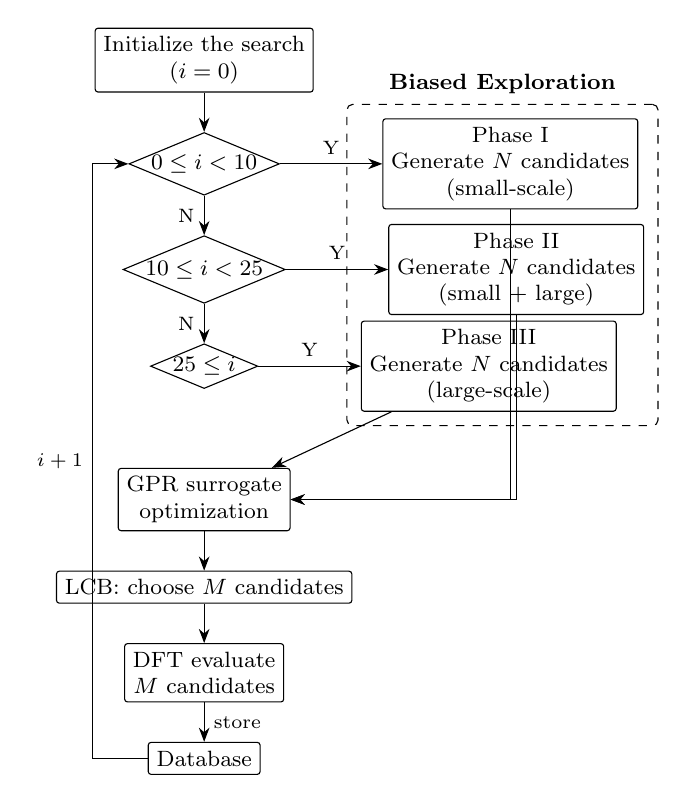
\begin{tikzpicture}[
  font=\footnotesize,
  >={Stealth[length=1.8mm]},
  node distance=5mm and 7mm,
  box/.style={draw, rounded corners=1pt, align=center, inner sep=3pt},
  dec/.style={draw, diamond, aspect=2.4, align=center, inner sep=0pt},
]
\node[box] (init) {Initialize the search\\ ($i = 0$)};
\node[dec, below=of init] (d1) {$0 \le i < 10$};
\node[dec, below=of d1] (d2) {$10 \le i < 25$};
\node[dec, below=of d2] (d3) {$25 \le i$};

\node[box, right=13mm of d1] (p1) {Phase I\\ Generate $N$ candidates\\ (small-scale)};
\node[box, right=13mm of d2] (p2) {Phase II\\ Generate $N$ candidates\\ (small $+$ large)};
\node[box, right=13mm of d3] (p3) {Phase III\\ Generate $N$ candidates\\ (large-scale)};

\begin{scope}[on background layer]
\node[draw, dashed, rounded corners=2pt, fit=(p1)(p2)(p3), inner sep=5pt] (BE) {};
\end{scope}
\node[above=0pt of BE.north, font=\footnotesize\bfseries] {Biased Exploration};

\node[box, below=10mm of d3] (gpr) {GPR surrogate\\ optimization};
\node[box, below=of gpr] (lcb) {LCB: choose $M$ candidates};
\node[box, below=of lcb] (dft) {DFT evaluate\\ $M$ candidates};
\node[box, below=of dft] (db) {Database};

\draw[->] (init) -- (d1);
\draw[->] (d1) -- node[left,font=\scriptsize]{N} (d2);
\draw[->] (d2) -- node[left,font=\scriptsize]{N} (d3);
\draw[->] (d1) -- node[above,font=\scriptsize]{Y} (p1);
\draw[->] (d2) -- node[above,font=\scriptsize]{Y} (p2);
\draw[->] (d3) -- node[above,font=\scriptsize]{Y} (p3);
\draw[->] (p1) |- (gpr);
\draw[->] (p2) |- (gpr);
\draw[->] (p3) -- (gpr);
\draw[->] (gpr) -- (lcb);
\draw[->] (lcb) -- (dft);
\draw[->] (dft) -- node[right,font=\scriptsize]{store} (db);
\draw[->] (db.west) -- ++(-7mm,0) |- node[pos=0.25,left,font=\scriptsize]{$i+1$} (d1.west);
\end{tikzpicture}
\caption{\label{fig:loop}The biased-exploration loop. Each iteration selects a phase from the
counter $i$, generates $N$ candidates with that phase's generator mix (Table~\ref{tab:schedule}),
optimises them against the GPR surrogate, ranks them with the LCB acquisition, evaluates the
selected candidates with DFT and stores them in the database; the counter then advances and the
phase is re-selected.}
\end{figure}

The early phases favour the small-scale (structure-aware) generator, which preserves the
layer-resolved character of the flat reference basin, while the later phases shift to the
large-scale rattle generator for broader exploration.

\subsubsection{Bias} The exploration is deliberately biased: the search is seeded from a
flat metal layer---the reference film geometry, a single-monolayer-thick film rather than a
random three-dimensional distribution of metal atoms---so the sampled database is a mixture of the
flat basin and any lower-lying basin the search finds. The composition of the reference layer
follows the target stoichiometry (Sec.~\ref{sec:models}): a pure Fe layer for Fe/MgO, and the same Fe
layer with B added above the surface for Fe-B/MgO. The films are single-layer in both models, and the
two reference layers differ only by the boron. Each model was run from multiple independent random
seeds, and each seed constitutes one independent search.

\subsubsection{Only completed searches are used} Every number in this paper comes from searches that ran
the full 100-iteration budget: 13 completed searches for Fe/MgO and 6 for Fe-B/MgO, 19 in
total. Two further searches were started and are \emph{not} used, and we record them here rather than
drop them silently---one Fe/MgO search reached only iteration 37, and one Fe-B/MgO search produced no
stored structures at all. A stopped search has had less search time than a completed one, so its best
energy is systematically worse; and because such searches are not distributed evenly across the two
models, including them would bias the comparison between them---as the method-parameter study in the
Supplementary Material also shows, where searches that stopped early inflate the mean of one setting
and depress another (Sec.~S3 of the Supplementary Material). The same criterion is applied without
exception throughout the analysis, and it is decided from the iteration count recorded for
each search, not from how a search is labelled: a search that looks complete can have stopped early,
and one whose stored structures are missing is treated the same way. In the two models used here the
excluded searches happen to be identifiable at a glance; the rule does not rely on that.

Candidates were relaxed by the surrogate model for up to 100 steps (starting from iteration 10) and
evaluated with the DFT calculator below. Only structures from iteration $\ge 10$ were used in
the analysis, i.e.\ after relaxation had begun; earlier pre-relaxation placements were discarded.

\subsection{DFT settings}
\label{sec:dft}

Energies and forces were obtained with GPAW \cite{gpaw2014} in linear combination of atomic orbitals
(LCAO) mode (double-zeta polarised basis), the Perdew--Burke--Ernzerhof (PBE) exchange--correlation
functional \cite{pbe1996}, a $(1\times1\times1)$ k-point mesh,
Fermi--Dirac smearing (width 0.05~eV), and spin polarisation with Hund's rule coupling enabled; a
Pulay mixer and a fixed convergence criterion (energy $10^{-4}$~eV, density/eigenstates $10^{-3}$)
were used throughout. Note the deliberately modest computational setup (single-layer slab,
$\Gamma$-point sampling): the study targets trends across compositions, not converged
absolute energies (see Sec.~\ref{sec:scope}).

The interfacial Fe--O separation is a construction parameter rather than a computed
quantity: the reference films are built with the first oxygen layer of the substrate 2.3~\AA{} above
the metal plane, and relaxation preserves that spacing (2.300~\AA{} for the flat basin, i.e.\
unchanged to the printed precision, and 2.331~\AA{} for the island). Comparison with the 2.0--2.3~\AA{}
range reported for this interface by low-energy electron diffraction (LEED) analyses and earlier
calculations
\cite{urano1988,butler2001} therefore checks the model construction rather than testing the
electronic-structure method. Independent of this, the LCAO basis set is appreciably less complete
than a plane-wave or real-space representation \cite{larsen2009}, so absolute geometric parameters
are reported at fixed settings and are not interpreted as converged values.

\subsection{Flatness and energy metrics}
\label{sec:metrics}

Two quantities describe each sampled structure:

Film flatness $\dZ$---the vertical span of the metal film,
$\dZ = z(\text{metal})_\text{max} - z(\text{metal})_\text{min}$, taken over the film's
metal atoms (Fe; boron is a metalloid and is not part of the flatness metric).
$\dZ \approx 0$ is a flat, wetting film; large $\dZ$ is a 3D island (dewetted). A threshold of
$\dZ \le 1.0$~\AA{} separates the ``flat'' and ``island'' basins.

Relative energy $dE/N$---the per-atom energy above the system's global minimum,
$dE/N = (E - E_\text{min})/N$, where $E_\text{min}$ is the lowest energy found for that composition
and $N$ the atom count. By construction the global minimum is $0$~\eVA; per-atom normalisation makes
the two models directly comparable despite their differing atom counts (75 and 78 atoms).

For each model, the flat-basin ground state (lowest $dE/N$ among $\dZ \le 1.0$~\AA{}
structures) was compared against the overall minimum, isolating the energy penalty of the flat
configuration.

\subsection{Robustness of the method}
\label{sec:robustness}

Because the search relies on a biased-exploration scheme, three method parameters were varied on the
Fe/MgO model to test robustness (Supplementary Material): the rattle strength, the LCB parameter
$\kappa$, and the inclusion of a dipole correction. The principal conclusion was shown to be
insensitive to $\kappa$ and to the dipole correction, and to degrade only when the rattle strength
was reduced. This is the same model, method and reference layer as the Fe/MgO results of
Sec.~\ref{sec:results}, so the study bounds the method used for the two models reported here.

\subsection{Scope and limitations}
\label{sec:scope}

The structures retained here are not DFT-converged minima: candidates were relaxed with the
surrogate model and evaluated with a single DFT step, leaving residual forces of order
1--2~eV/\AA. Accordingly, ``lowest energy'' and ``basin'' denote the lowest DFT energy
\emph{encountered} in the search, not a converged minimum, and the results are interpreted
qualitatively (trends across compositions). The flat configuration is therefore described as a
\emph{higher-energy flat basin}, not as a metastable state---establishing metastability would require
converged relaxations, a Hessian (no imaginary modes) and a barrier between basins. A full
re-relaxation of representative structures is necessary for this purpose.

The models additionally build both phases on a body-centred cubic (bcc) Fe lattice, whereas the
experimentally reported structure of ultrathin Fe on MgO(001) is body-centred tetragonal
below about 10~\AA, changing to bcc only above that thickness \cite{urano1988}. The island branch
spans $\dZ \approx 1$--$6$~\AA, so the structures compared here lie in the thickness regime in which
the experimental film is not bcc. The flat--island comparison should therefore be read as a trend
obtained within a fixed lattice model, not as a prediction of absolute structural parameters.

One further property of the model bounds its interpretation: the strain convention is the
inverse of the experimental stack. The simulation cell takes the Fe lattice constant and the
substrate is compressed to match it, so the Fe film is unstrained in-plane, whereas in a
real junction a thin Fe film on bulk MgO absorbs the mismatch as in-plane strain and relieves it
through interfacial dislocations. This model therefore does not represent the strained-film
situation (see Sec.~\ref{sec:limitations}). The convention is the same for both models reported
here, so it does not enter the Fe/MgO-vs-Fe-B/MgO comparison at all.

Finally, the two models differ \emph{only} by the added boron: both are built on the same lattice
constant, the same substrate, the same reference-layer geometry and the same candidate-generation
schedule. What the comparison cannot separate is boron from \emph{any} added element---a second,
chemically different film composition would be needed for that, and none is analysed here.

% Ported from sections/02_results.md (v6, APPROVED 2026-09-18).
% Final-manuscript Sec.~III. Floats: Table 3, Table 4, Figure 2, Figure 3.
\section{Results}
\label{sec:results}

\subsection{The two-phase landscape of the metal film on MgO}
\label{sec:landscape}

Our target is the wetting of the metal film on MgO(001). The property that distinguishes a wetting
from a dewetting film is its flatness, measured by the vertical span of the film,
$\dZ = z(\text{metal})_\text{max} - z(\text{metal})_\text{min}$ over the film's metal atoms (Fe);
$\dZ \approx 0$ is a flat, wetting film and large $\dZ$ a three-dimensional island. We therefore
designed the search to return a map of this two-phase landscape: a GOFEE global optimisation
(Sec.~\ref{sec:bias}) seeded from a flat reference layer, so that the flat basin is
populated from the outset and any lower-lying basin the search finds is populated alongside it. The
result is a sampled distribution over $\dZ$ and energy---an \emph{exploration} density, not a
thermodynamic density of states. Because the sampling is deliberately biased, we use it only for
unweighted structural and energetic comparisons; the number of structures in a basin is a descriptive
attribute of the sampled database, not a physical population.

Across the two models the search returns 1723 structures spanning $\dZ$ from 0.001 to 5.57~\AA,
with both phases populated in each (Table~\ref{tab:phases}). Fig.~\ref{fig:landscape} draws that
landscape: every structure is placed at its own vertical span and at its energy above the model's
lowest, so the figure is the map the search was designed to produce rather than a selection of
representative structures. The points form a continuous band that descends from the flat window into
an island minimum near $\dZ = 3.7$~\AA{} in both models, and the two panels share one energy scale,
so a given height means the same relative energy in either.

\begin{table}[t]
\small
\caption{\label{tab:phases}The two phases in each model ($\dZ \le 1.0$~\AA{} $=$ flat/wetting;
$\dZ > 1.0$~\AA{} $=$ island).}
\begin{tabular*}{\textwidth}{@{\extracolsep{\fill}}lccccc}
\toprule
Model & Structures & Island & Flat & Global-min $\dZ$ (\AA) & Flat-basin min $dE/N$ (\eVA) \\
\midrule
Fe/MgO   & 1180 & 985 & 195 & 3.65 & 0.1888 \\
Fe-B/MgO & 543  & 430 & 113 & 3.77 & 0.1493 \\
\bottomrule
\end{tabular*}
\end{table}

\begin{figure}[t]
\centering
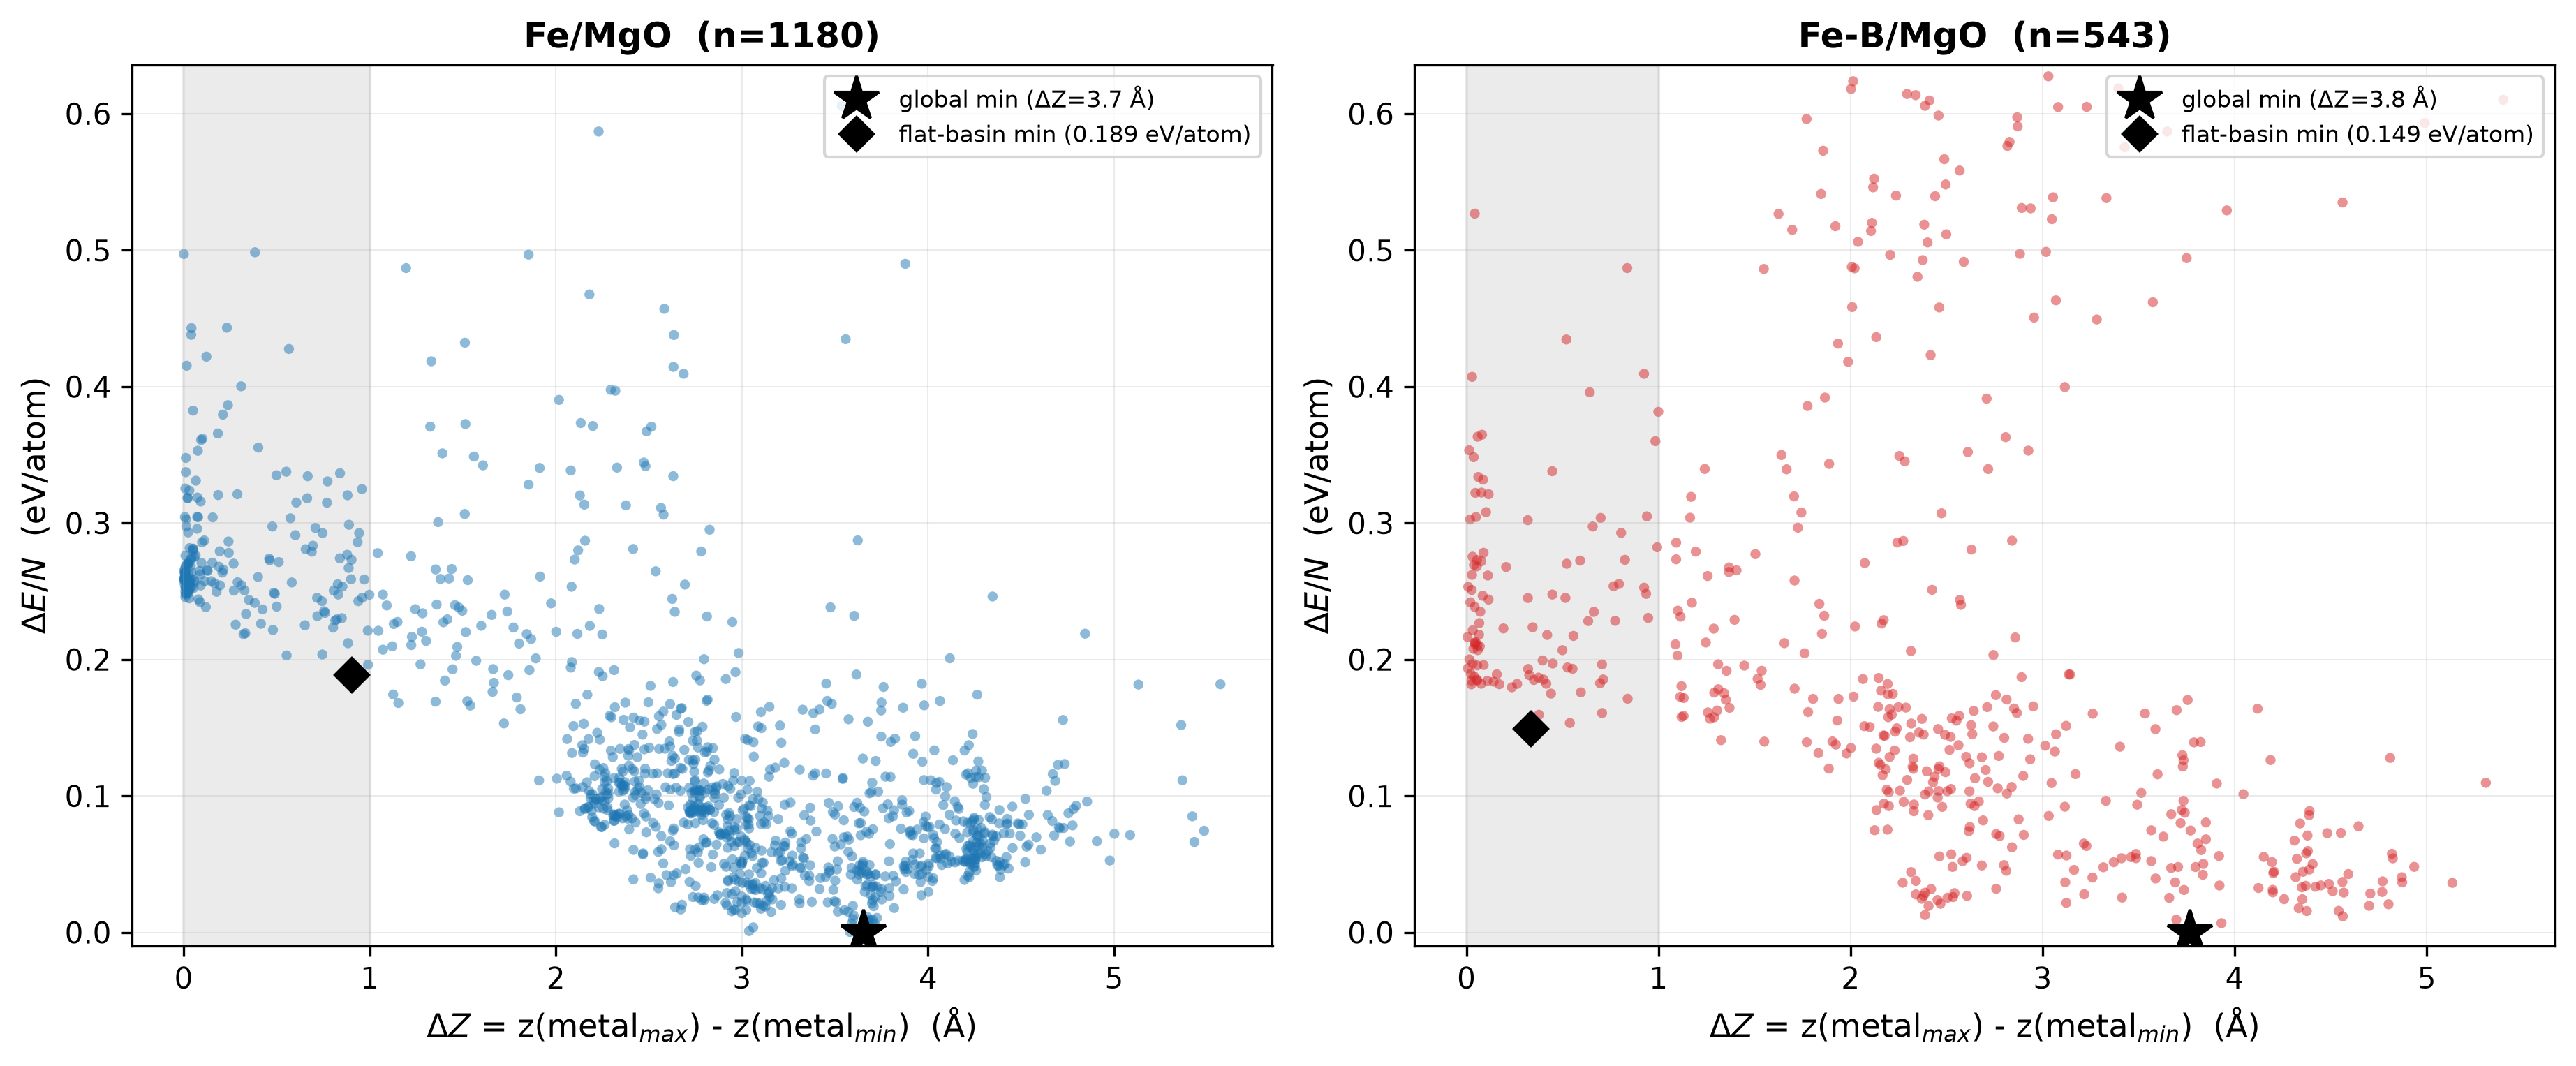
\includegraphics[width=\textwidth]{pes_2_systems.png}
\caption{\label{fig:landscape}The sampled two-phase landscape of the metal film on MgO. Each point is
one structure from the Fe/MgO (left) and Fe-B/MgO (right) searches, plotted as its relative energy
$dE/N$ above the model's own lowest energy against the vertical span of the film, $\dZ$. The shaded
band is the flat window ($\dZ \le 1.0$~\AA); the star marks the model's lowest-energy structure and
the diamond the best member of its flat basin. Both panels use the same energy scale.}
\end{figure}

\subsubsection{The island is the ground state in both models, despite the flat bias} The lowest-energy
structure found is an island in each model, with its global minimum at $\dZ = 3.65$~\AA{} (Fe/MgO)
and 3.77~\AA{} (Fe-B/MgO) (Table~\ref{tab:phases}, column 5)---a three-dimensional cluster rather
than a flat film. This result is \emph{against} the direction of the bias: every search was seeded
from a flat reference layer and, in the early phases, perturbed only at small scale from it, so the
flat configuration had a systematic head start. The search nevertheless left the flat basin and
converged on an island in both models. The flat-wetting state is therefore not an artefact of how the
initial structures were built---it is genuinely higher in energy than the island.

\subsubsection{The flat configuration is a distinct, higher-energy basin} Taking for each model the
lowest-energy structure with $\dZ \le 1.0$~\AA{} isolates the flat basin's best member. In both
models it lies above the global minimum---by 0.1888~\eVA{} for Fe/MgO and 0.1493~\eVA{} for
Fe-B/MgO (Table~\ref{tab:phases}, column 6). The flat film is thus a separate basin of the
landscape, not merely the high-$\dZ$ tail of a single minimum.

\subsubsection{The branches are families, not single structures} The $\dZ$ values are continuous rather
than grouped into discrete island heights: in each model the island branch spans $\dZ \approx
1$--$5.6$~\AA{} with a median of 3.02~\AA{} (Fe/MgO) and 2.58~\AA{} (Fe-B/MgO), and the flat branch
spans the whole window below 1~\AA. The low-energy members of each branch are likewise not a single
repeated structure: comparing the lowest-energy structures of each branch by their radial/angular
fingerprint shows that each branch's low-energy set splits into two distinct structural
motifs, and that a motif recurs across independent searches---for Fe/MgO, the five lowest flat
structures come from five different searches and fall into two motifs, four of them in the dominant
one.
The fingerprint is computed on the whole template-plus-film structure, so the fixed MgO template
compresses the pair distances and the motif count is a lower bound on the structural
diversity present; a film-resolved descriptor would be sharper. Pairwise distances within the
low-energy set of a branch are 0.41--0.44 of that branch's random-pair distance scale, i.e.\ the
low-energy structures are consistently more compact than the branch as a whole. The count is also
limited by how many searches contribute to the low-energy set: the Fe-B/MgO flat set within
0.02~\eVA{} of its minimum comes from two searches and its island set from three, so those counts
rest on fewer independent searches than the corresponding Fe/MgO numbers (five and four).

\subsubsection{Experimental correspondence} The films in this study are about one monolayer thick
on average---25 metal atoms per 25 substrate sites in the $5\times5$ cell, the boron-containing film
carrying three additional boron atoms---and that is the regime in which the growth mode of Fe on
MgO(001) has been characterised experimentally. At room temperature the observed growth is
three-dimensional: He-atom scattering shows 3D metal island growth of Fe on MgO(001), with
quantified island densities, sizes and shapes, suppressed only when the film is deposited at low
temperature (140~K), where a monolayer almost completely covers the substrate \cite{fahsold2000};
scanning tunnelling microscopy finds that sub-nanometre Fe grows three-dimensionally on MgO,
with island coalescence between 3.5 and 6.5 monolayers and a two-dimensional growth mode reported
only above $\approx$6.5 monolayers \cite{torelli2009}; and grazing-incidence small-angle X-ray
scattering on five monolayers evaporated at room temperature likewise identifies Volmer--Weber
growth with spherical islands \cite{reitinger2007}. A flat, continuous film is obtained instead by
low-temperature deposition \cite{fahsold2000} or by slow deposition onto a cleaved, oxygen-annealed
crystal, where the first monolayer grows pseudomorphically and layer by layer \cite{urano1988}. Our
two basins therefore map onto the two outcomes that are experimentally accessible at this
coverage---the flat basin onto the pseudomorphic monolayer and the island basin onto the 3D
clusters---and the energy ordering we find places the flat, wetting configuration above the island.
This is a consistency check rather than a prediction: the observed growth mode is also set by
kinetics, so the correspondence is between structural configurations, not between energies. Because
the growth mode turns two-dimensional only above $\approx$6.5 monolayers \cite{torelli2009}, the
comparison is specific to the monolayer regime and should not be extrapolated to thick films.

\subsection{The flat (wetting) phase with and without boron}
\label{sec:flat}

With the two phases established, we compare how adding boron to the Fe film shifts the flat basin.
Table~\ref{tab:flatbasin} gives the flat-basin minimum $dE/N$ for the two models, i.e.\ the same host
with and without the metalloid, and Fig.~\ref{fig:flat} places the two values side by side with the
change between them marked.

\begin{table}[t]
\small
\caption{\label{tab:flatbasin}Flat-basin minimum $dE/N$ (\eVA) for the same Fe host with and
without boron.}
\begin{tabular*}{\textwidth}{@{\extracolsep{\fill}}lcc}
\toprule
Film & Flat-basin min $dE/N$ (\eVA) & B effect \\
\midrule
Fe   & 0.1888 & --- \\
Fe-B & 0.1493 & \textbf{$-0.040$} \\
\bottomrule
\end{tabular*}
\end{table}

\begin{figure}[t]
\centering
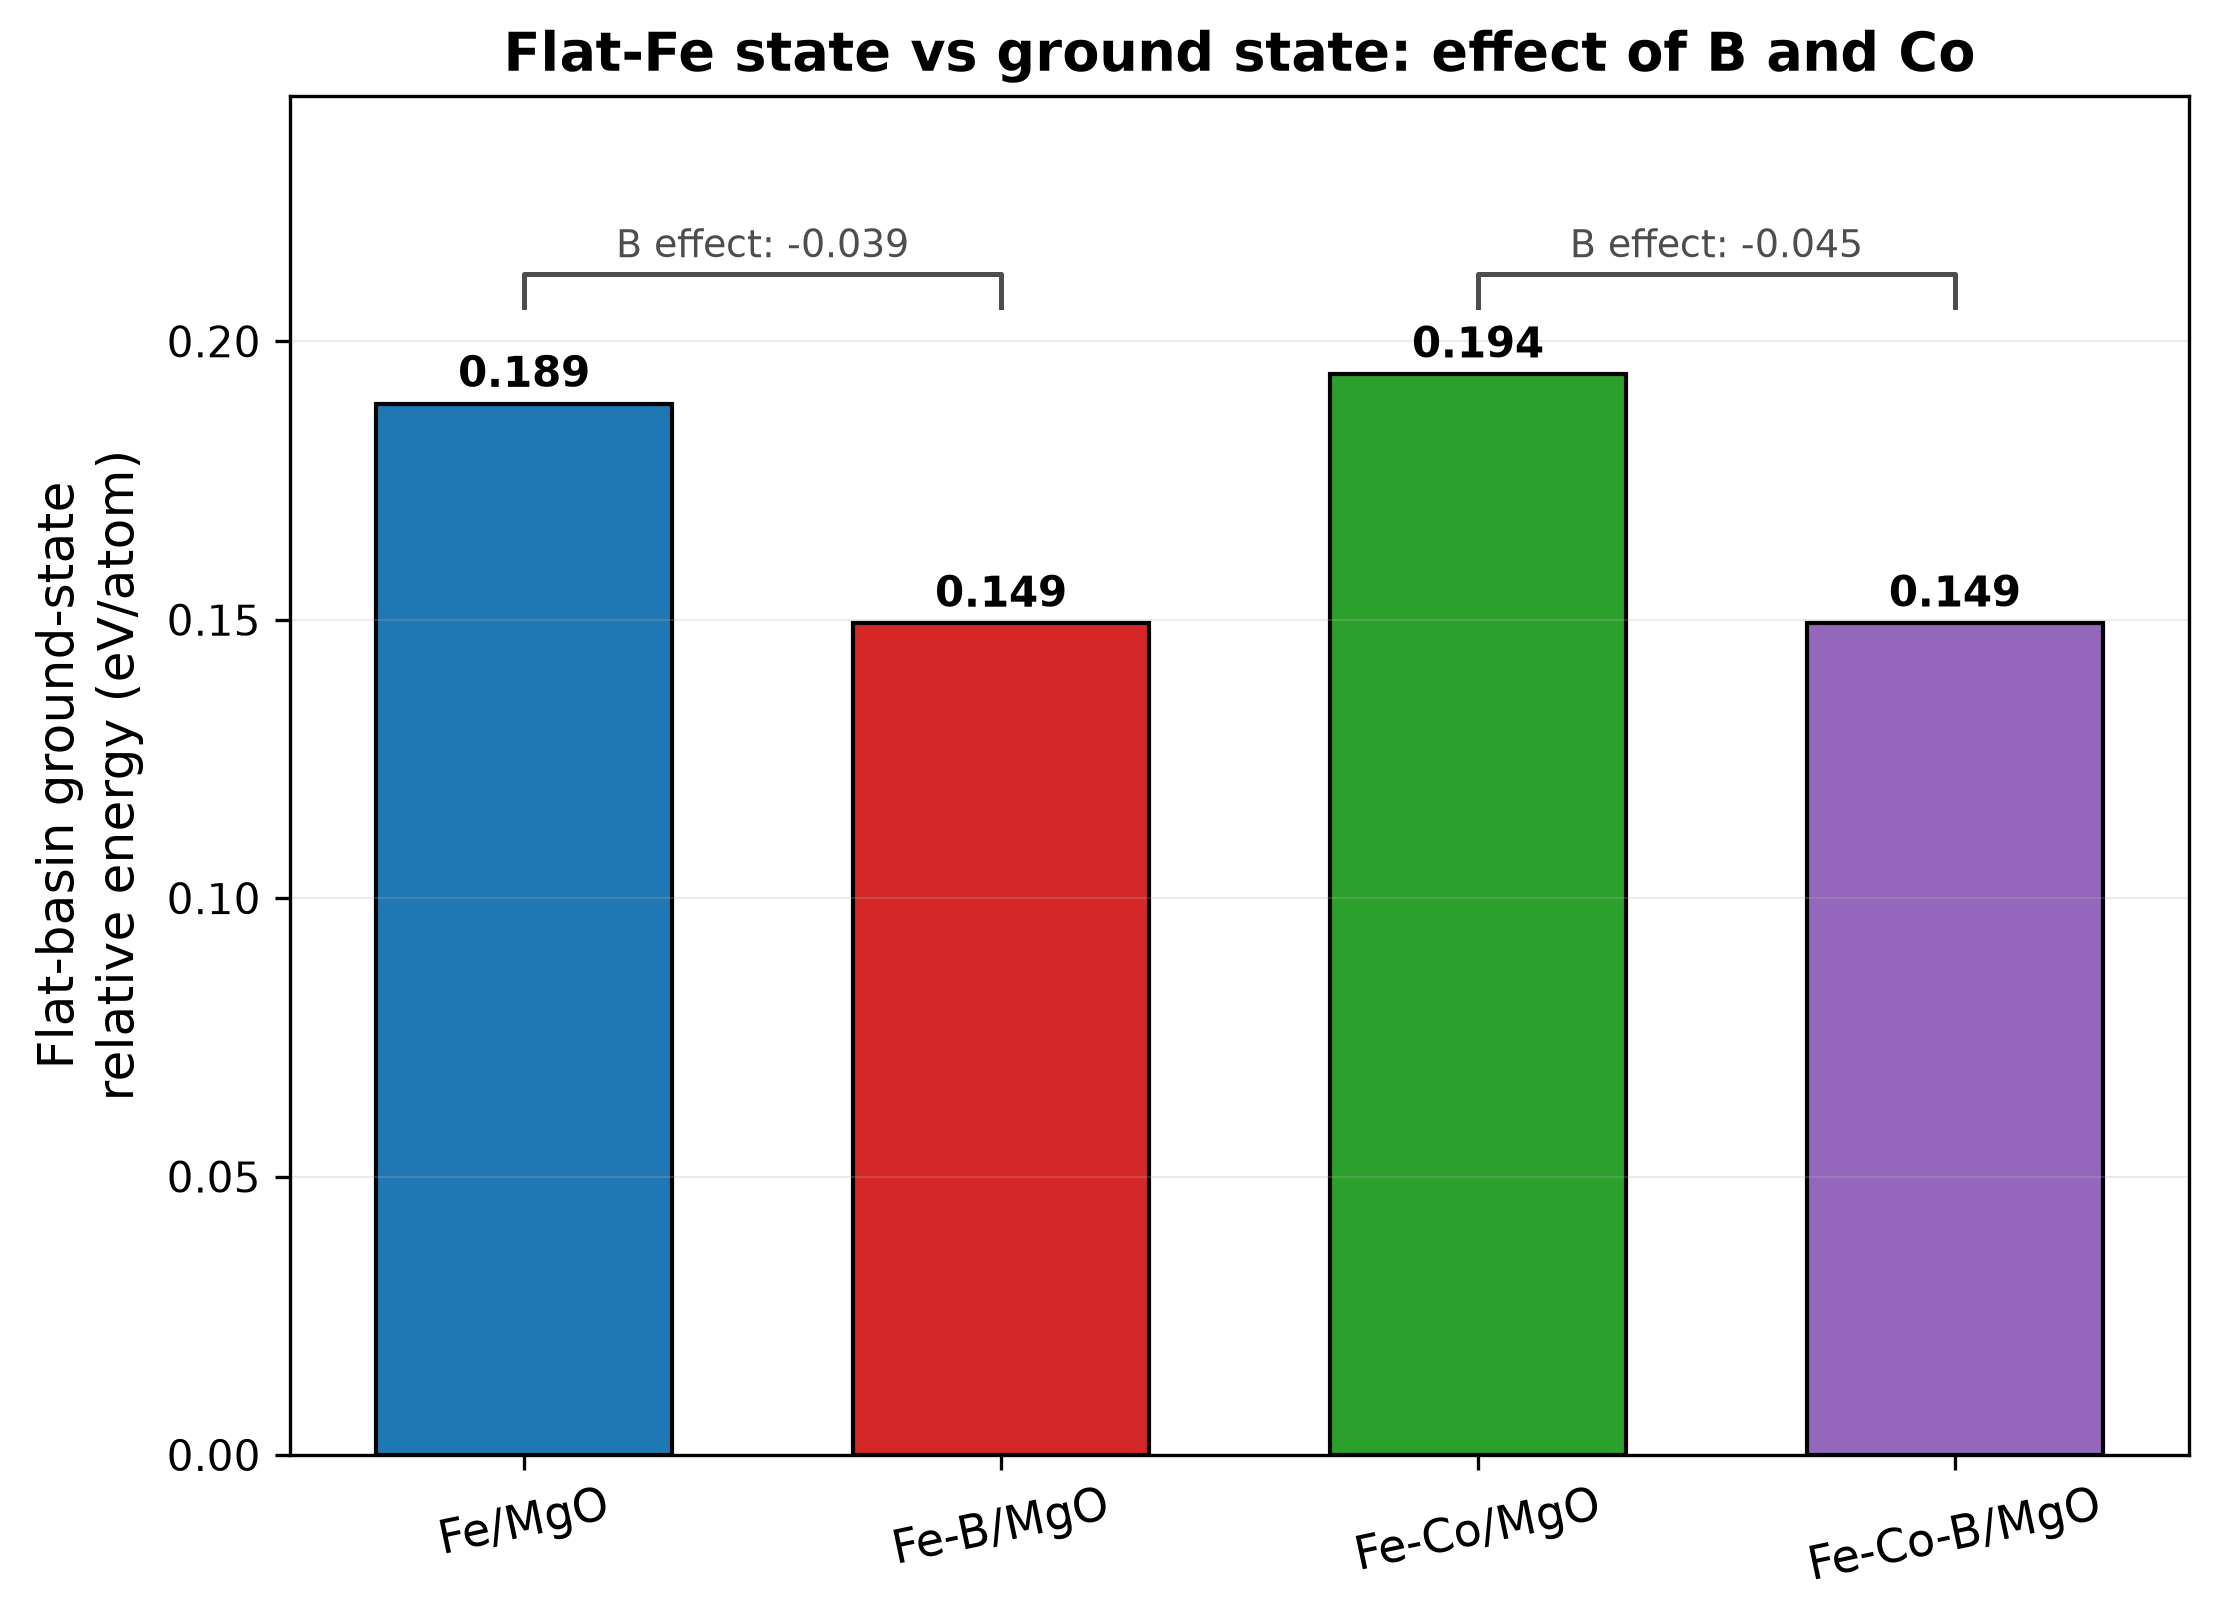
\includegraphics[width=\textwidth]{flat_state_summary.png}
\caption{\label{fig:flat}Flat-basin minimum relative energy for the same Fe host with and without
boron. A bar is the lowest energy found among the structures of the flat window ($\dZ \le 1.0$~\AA),
in \eVA{} above the model's own lowest energy, and the bracket gives the shift produced by boron.}
\end{figure}

\subsubsection{Boron lowers the flat-state energy} Adding boron lowers the flat basin's best member by
0.040~\eVA---from 0.1888 to 0.1493~\eVA---a 21\,\% reduction of the flat--island separation.
The effect is measured across 13 independent Fe/MgO searches and 6 independent Fe-B/MgO searches; its
search-level significance is given in the uncertainty paragraph below.

\subsubsection{Boron does not bond to the MgO interface} Restricting to the low-energy window
($dE/N \le 0.05$~\eVA), only 1 of the 72 Fe-B/MgO structures in that window has any boron atom within
2.6~\AA{} of an oxygen of the substrate; the maximum boron--oxygen contact fraction in the window is
0.33. Outside the window the picture is different---101 of the 471 remaining Fe-B/MgO structures do
have a boron--oxygen contact---which is why the statement is restricted to the low-energy window
rather than made over all sampled structures. Boron therefore remains inside the metal film rather
than wetting the oxide, so its effect on the flat phase is film-internal rather than a change in
interfacial bonding.

\subsubsection{Uncertainty from the choice of search} Each model was searched from several independent
random seeds (13 completed searches for Fe/MgO, 6 for Fe-B/MgO), and structures from one search are
correlated with each other, so the independent unit is the search, not the structure. Taking each
search's own flat-basin minimum, the per-search minimum falls from 0.2171~\eVA{} without boron to
0.1882~\eVA{} with it on average (medians 0.2185 and 0.1834), a median shift of
0.0351~\eVA{} with 94\,\% of resampled replicates agreeing in sign---the effect is not carried by a
single favourable search, and the best-structure difference of Table~\ref{tab:flatbasin}
($-0.040$~\eVA) is the extreme of the same distribution rather than a lone outlier. A two-sided
permutation test over the 19 searches gives $p = 0.0444$, significant at the 5\,\% level. In
words, $p$ is the probability that a random reshuffling of the 19 per-search minima into two groups
of 13 and 6 would, by chance alone, produce a shift in the flat-state energy at least as large as the
one observed---so $p = 0.0444$ means such a shift arises by chance in only about 4.4\,\% of
reshufflings, i.e.\ the observed lowering of the flat state is unlikely to be a chance outcome of
which searches happened to contain boron. The test is an exact enumeration of all 27\,132
partitions of the pooled search minima, so this value is exact for the data and its resolution floor
is $p = 3.7\times10^{-5}$---more than three orders of magnitude below the value reported, i.e.\ the
conclusion is not an artefact of too few searches.

\subsection{The island (dewetting) phase and the separation between phases}
\label{sec:island}

Adding boron leaves the \emph{island} phase qualitatively similar. In both models the lowest-energy
structure is an island---at $\dZ = 3.65$~\AA{} (Fe/MgO) and 3.77~\AA{} (Fe-B/MgO)
(Table~\ref{tab:phases})---and the island branch spans the same broad range of heights in both
($\dZ \approx 1$--$5.6$~\AA, median 3.02~\AA{} without boron and 2.58~\AA{} with it). Boron does not
change what the dewetted state looks like; it changes how far above it the flat, wetting state sits.

Because each model is referenced to its own lowest energy, the quantity that compares the two phases
is the separation between them---the flat-basin minimum of Table~\ref{tab:flatbasin}---and
that separation is what boron reduces. The present data do not resolve \emph{how} boron reduces it: a
lower flat-basin energy could equally arise from stabilising the flat phase or from destabilising the
island, and distinguishing the two would require the island phase to be referenced to an absolute
(rather than per-model) energy scale, or a converged treatment of both basins. We therefore state the
effect as a change in the flat--island separation, not as the stabilisation of either phase
individually.

\subsection{Summary of the results}
\label{sec:summary}

The biased GOFEE search, seeded from a flat reference, maps both the flat (wetting) and island
(dewetting) phases in both models, over $\dZ = 0.001$--$5.57$~\AA. The island is the ground state in
both models ($\dZ = 3.65$ and 3.77~\AA), even though the search was biased toward the flat
configuration---the flat bias did not manufacture the result---and the flat configuration is a
distinct, higher-energy basin, 0.1888~\eVA{} above the island for Fe/MgO and 0.1493~\eVA{} for
Fe-B/MgO, in both cases a separate basin rather than the high-$\dZ$ tail of a single minimum. Boron
lowers the flat--island separation by 0.040~\eVA{} (13 vs 6 completed searches, exact two-sided
permutation $p = 0.0444$) without displacing the island as the ground state, and it does not bond to
the MgO interface---it stays within the film, so its effect on the flat phase is film-internal.

The low-energy structures of each branch form a small set of recurring motifs rather than one
repeated structure, and $\dZ$ is continuous: the two phases are families, and the energetics above
are compared unweighted, since the sampled densities are biased and not physical.

The mechanistic origin of these trends (electronic structure, interface registry) and the robustness
of the method to its parameters are presented in the Supplementary Material.

% Ported from sections/03_discussion.md (v5, APPROVED 2026-09-18).
% Final-manuscript Sec.~IV.
\section{Discussion}
\label{sec:discussion}

\subsection{Why the island is the ground state}
\label{sec:island-ground}

The search finds an island ground state in both models, with the flat film sitting 0.19~\eVA{} higher
for Fe/MgO and 0.15~\eVA{} higher for Fe-B/MgO. The electronic-structure analysis (Supplementary
Material) indicates why. In the flat monolayer every metal atom is registry-locked directly atop an
oxygen of the MgO surface---the registry of the reference construction, and the one determined
experimentally for the first monolayer of Fe on MgO(001) by LEED I--V analysis \cite{urano1988} and
used in first-principles models of the Fe$|$MgO$|$Fe interface \cite{butler2001}---maximising Fe--O
orbital overlap and pushing the Fe $d$-band centre down to $-0.23$~eV. The island abandons that
registry: the number of metal atoms registered directly atop an oxygen drops from 25 (of 25) to 9 (of
25), the island's interface Fe $d$-band centre rises to $+0.51$~eV ($+0.60$~eV averaged over all
island Fe), and the film becomes electronically ``quieter'' (lower DOS at the Fermi level, weaker
spin polarisation). The island's energy gain is therefore dominated by \textbf{reduced forced
interfacial coupling and restored metal cohesion}: the registry-locked monolayer spends its bonding
on Fe--O contacts while forgoing the three-dimensional Fe--Fe coordination available to a cluster,
and the island reverses that trade.

It is \textbf{not} a lattice-strain effect. The in-plane mismatch of this interface (3.6\,\% of the
MgO lattice against the Fe lattice, Sec.~\ref{sec:models}) is carried by the \textbf{substrate},
which is built in that compressed state and held fixed, not by the film; the Fe film sits at its own
equilibrium lattice constant and is not strained in-plane, so there is no film strain for the island
to relieve. The mechanism is consistent with the weak Fe--MgO coupling found in first-principles
treatments of the interface \cite{butler2001}, and with the experimental observation that a flat
monolayer requires low-temperature or slow deposition while room-temperature growth gives 3D islands
at the same one-monolayer coverage \cite{fahsold2000,torelli2009,reitinger2007}.

\subsection{Why boron stabilises the flat film}
\label{sec:boron}

Boron lowers the flat-state energy by 0.040~\eVA, bringing the flat configuration closer to the
ground state. Two observations frame the mechanism. First, boron does \textbf{not} bond to the MgO
interface---it remains inside the metal film (a single B--O contact in one of 72 windowed Fe-B
structures)---so its effect is not interfacial. Second, the shift is not carried by one favourable
search: the Fe-B model's six per-search flat minima lie between 0.1493 and 0.2481~\eVA, five of them
below the Fe host's median of 0.2185~\eVA, and 94\,\% of resampled replicates agree in sign
(Sec.~\ref{sec:flat}). Both observations point to an intrinsic, film-internal role for boron rather
than an interfacial or statistical one.

\textbf{Confusion principle and amorphous formation.} The flat film can be read as the disordered,
amorphous-like configuration and the island as the ordered, crystalline-like one. Under this reading,
the stabilisation of the flat state by added elements follows the \textbf{confusion principle} of
metallic-glass formation \cite{greer1993}: the more elements in an alloy, the harder it is for the
alloy to select a viable crystal structure, and the greater the tendency toward glass (amorphous)
formation.

Our results are partly consistent with this. Adding boron lowers the flat-basin energy
($0.1888 \to 0.1493$~\eVA), i.e.\ the added element stabilises the disordered configuration relative
to the ordered one, in the direction the principle predicts. The present models test this for a
single added metalloid and cannot decide between the competing readings of the principle---whether it
acts through the \emph{presence of an added species} by a film-internal mechanism, or through the
\emph{number} of species, which would require the same host with two different additions to separate.
We therefore read our result as consistent with the confusion principle acting through the added
metalloid and leave the element-count reading untested here (see Sec.~\ref{sec:limitations}).

We note, however, that the boron-containing film retains the island as its ground state---the
confusion principle stabilises the flat state but does not, in this small model system, fully
suppress the ordered configuration. The precise origin of boron's effect---whether it lowers the flat
basin's energy or raises the island's---is not resolved by the present data and is a natural target
for the re-relaxation and further analysis.

\subsection{Implications for MTJ stacks}
\label{sec:mtj}

The performance of MgO-based magnetic tunnel junctions rests on the structural quality of the
metal/oxide interface. The giant tunnel magnetoresistance of single-crystal Fe/MgO/Fe junctions
arises from coherent spin-polarised tunnelling across a lattice-matched interface, with the residual
mismatch accommodated by interfacial dislocations and the growth conditions chosen to minimise them
\cite{yuasa2004}. The present results connect to this in two ways. First, they show that a perfectly
flat, registry-locked metal layer maximises Fe--O bonding at the expense of metal coordination and is
therefore energetically penalised relative to a clustered film---a consideration for interface
engineering in MgO-based tunnel junctions, whose barrier must stay flat and coherently matched for
the tunnelling magnetoresistance to reach its high values \cite{yuasa2004}. Second, they show that
boron acts to stabilise the flat configuration without bonding to the interface, consistent with the
picture of boron as a film-internal agent that promotes a flat, well-wetting interface.
These are trend-level, model-system conclusions; quantitative transfer to a device stack would
require the converged relaxations and a fuller treatment of the interface.

\subsection{Limitations}
\label{sec:limitations}

One scope bound follows from the design rather than from the methods. The paper compares a single
host with and without one added element, boron. Nothing here separates the effect of \emph{boron}
from the effect of \emph{an added element as such}; that would need a second chemically different
addition in the same host, which is not analysed (the element-count reading of the confusion
principle is therefore untested---Sec.~\ref{sec:boron}). What the design does exclude is a trivial
explanation from the construction: the two models share the lattice constant, substrate,
reference-layer geometry and candidate-generation schedule, and differ only by the boron
(Sec.~\ref{sec:scope}).

The results are qualitative/trend-level: the structures are not DFT-converged minima (residual
forces $\sim$1--2~eV/\AA), the models are single-layer slabs at $\Gamma$-point sampling, and the
flat/island split uses a chosen $\dZ$ threshold. The two models also have unequal seed counts (13
completed searches for Fe/MgO against 6 for Fe-B/MgO) and their atom counts differ (75 and 78), so
sampling fractions are compared only as trends, not as like-for-like populations. The flat state is
described as a higher-energy configuration, not a proven metastable state. A full re-relaxation of
representative structures is necessary to place these conclusions on converged minima.

Two features of the model itself bound the interpretation. First, the \textbf{strain convention is
the inverse of the experimental stack}: here the in-plane lattice is the Fe lattice constant and the
\textbf{MgO substrate} is the compressed component, held fixed, whereas in a real junction the bulk
MgO imposes its lattice on a thin Fe film, which absorbs the mismatch as in-plane strain and relieves
it through interfacial dislocations \cite{yuasa2004}. The film in this work is therefore unstrained,
and this model does not represent the strained-film situation. Second, both phases are built on a
body-centred-cubic Fe lattice, while the experimentally reported structure of ultrathin Fe on
MgO(001) is body-centred tetragonal below about 10~\AA{} \cite{urano1988}; the island branch
($\dZ \approx 1$--$5.6$~\AA) lies in that regime (Sec.~\ref{sec:scope}). The flat--island comparison
is therefore a trend obtained within one fixed lattice model, and extending it to thicker,
experimentally strained films would require a different construction.

\textbf{The search-level statistic rests on 19 searches, and it is asymmetric.} The comparison pools
13 completed searches of the Fe/MgO model against 6 of the Fe-B/MgO model. The permutation test
enumerates all 27\,132 partitions of that pool, so its resolution floor is $p = 3.7\times10^{-5}$ and
the reported $p = 0.0444$ is not limited by the number of searches; it would, however, tighten with
more completed Fe-B/MgO searches, since the smaller group sets the width of the null. Two further
bounds follow from the same asymmetry. The boron-free interface statement (Sec.~\ref{sec:flat}) is
measured on the 72 Fe-B/MgO structures inside the low-energy window, which come from \textbf{four} of
the six searches---so its effective number of independent observations is closer to four than to
72---and the Fe-B/MgO motif counts (Sec.~\ref{sec:landscape}) rest on two (flat) and three (island)
searches against five and four for Fe/MgO. Statements resting on those sets are correspondingly
weaker evidence than the flat-basin energies of Table~\ref{tab:flatbasin}, which use every search of
both models.

% Ported from sections/05_conclusion.md (v2, APPROVED 2026-09-18).
% Final-manuscript Sec.~V. Cites greer1993.
\section{Conclusion}
\label{sec:conclusion}

We studied the wetting of a metal film on MgO(001)---the interface at the heart of MgO-based magnetic
tunnel junctions---for the same Fe host with and without added boron. Using a biased,
surrogate-driven search that targets the two configurations the wetting question is about, we mapped
the landscape into its two growth modes: a flat, well-wetting film and a dewetted island. In both
models the island is the ground state, so the flat film is a distinct, higher-energy basin---by
0.1888~\eVA{} for Fe/MgO and by 0.1493~\eVA{} for Fe-B/MgO. Adding boron lowers the flat--island
separation by 0.040~\eVA, a 21\,\% reduction, at a search-level significance of $p = 0.0444$---the
fraction of random relabellings of the 19 searches that would reproduce a shift this large if boron
had no effect. Boron acts inside the film rather than at the interface, and it does not displace the
island as the ground state: the ordered, three-dimensional configuration remains the more stable of
the two in both models.

Boron insertion therefore lowers the relative energy of the flat, well-wetting configuration, moving
it closer to the island ground state without displacing it. This is the direction the confusion
principle of metallic-glass formation predicts---an added element stabilises the disordered, flat
configuration relative to the ordered one \cite{greer1993}---and it matters for MgO-based tunnel
junctions, whose performance depends on a flat, coherent metal film on the barrier. The metal film's
tendency to dewet into islands at monolayer coverage, and the control of interface flatness that
modern junction fabrication demands, make the energetic balance between these two configurations a
quantity worth knowing.


\bibliographystyle{unsrtnat}
\bibliography{references}

\end{document}
